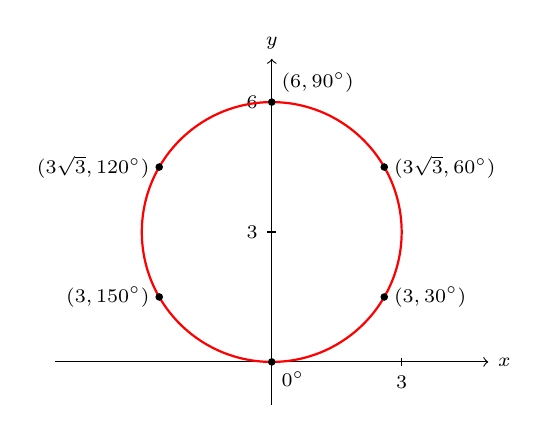
\begin{tikzpicture}[scale=0.55, every node/.style={font=\scriptsize}]
  \draw[->] (-5,0) -- (5,0) node[right] {$x$};
  \draw[->] (0,-1) -- (0,7) node[above] {$y$};
  \foreach \x in {3} \draw (\x,0.1) -- (\x,-0.1) node[below] {$\x$};
  \foreach \y in {3,6} \draw (0.1,\y) -- (-0.1,\y) node[left] {$\y$};
  \draw[red, thick] (0,3) circle (3);
  \foreach \a/\lab/\pos in {0/{0^\circ}/below right, 30/{(3,30^\circ)}/right, 60/{(3\sqrt3,60^\circ)}/right, 90/{(6,90^\circ)}/above right, 120/{(3\sqrt3,120^\circ)}/left, 150/{(3,150^\circ)}/left} {
    \fill (\a:{6*sin(\a)}) circle (2.5pt) node[\pos] {$\lab$};
  }
\end{tikzpicture}
